CPU speeds are usually measured by timing the execution time of programs. Since
a computer program is just a collection instructions, the speed of the CPU is
determined by how fast it can process each instruction.
Every CPU has a clock, which ticks at a given rate. For every tick, a new
instruction is executed. This clock ensures that all instructions "flow" through
the processor without problems, and that the electrical components, such as the
ALU or the control-unit, can manage to carry out their tasks in that time.
Naturally, electrical engineers have pushed the limits of the circuits to manage
the highest clock rate. The clock rate of the very first processors was measured
in hertz and kiloHertz (kHz), but most modern desktop CPUs reach in multiple
GigaHertz (GHz)\cite{wiki:clock_rate}. However, even with those speeds, the
demand for faster processing units is ever-growing, and other techniques to speed-up
the execution are used.\\
One of those techniques is pipelining, which separates the circuit into multiple
stages, much like the assembly lines in factories. In such factories, workers
have their own station at the assembly line, do a specific task repeatedly, and
forward it down the line. This greatly increases the throughput of a factory and
decreases the labor need.
In MIPS, this idea is implemented by separating the processor into 5 stages\cite{COD5}:
\begin{itemize}
	\item Instruction Fetch (IF)\\
Fetches the next instruction.

	\item Instruction Decode (ID)\\
Reads the instruction, sets the appropriate control flags, reads the relevant
registers and sends the data to the next stage.

	\item Execute (EX)\\
Executes the instruction. This is typically done by the ALU with the appropriate
operation supplied.

	\item Memory Access (M/MEM)\\
All operations on memory happen here. This stage either loads a memory address
or stores a value at an appropriate address.

	\item Write Back (WB)\\
Writes the results to the CPU registers.
\end{itemize}
Each of these stages will naturally use less time than all of them combined, and
since the clock is shared in all stages, it is set to the slowest stage in the
pipeline.\\
Not only do we have faster tick rate on our clock, but we are also able to
perform multiple operations concurrently. Figures \ref{fig:single_cycle_time}
and \ref{fig:pipeline_time} show the timing of each instruction, and how
pipelining might improve the whole process.
\begin{figure}[H]
        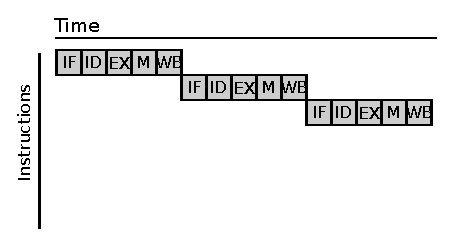
\includegraphics{pipeline/single_cycle.eps}
	\caption{Single cycle implementation.}
        \label{fig:single_cycle_time}
\end{figure}
\begin{figure}[H]
        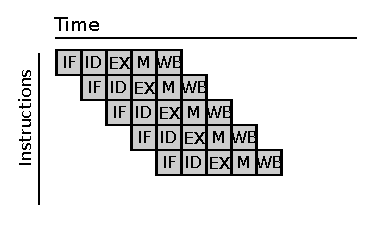
\includegraphics{pipeline/pipeline.eps}
	\caption{Pipelined approach.}
        \label{fig:pipeline_time}
\end{figure}


\subsection{Design of the MIPS32 Pipeline}
The advantages of a pipelined design does not come without a price. Although
the single-cycle implementation of the processor is very similar to the
pipelined approach, it has its fair sets of challenges. The main problem with
executing instructions concurrently is that the instructions will often rely on
the result of the previous instructions. These situations are referred to as
hazards.

\subsubsection{Data Hazard}
Data hazards mainly occur when an instruction cannot continue, because it must
wait for the result from an earlier instruction. Suppose a program wants to
calculate the sum of 4 integers:
$$A = A + B + C + D$$
In MIPS32 assembly, this would be written as:
\begin{figure}[H]
	\centering
	\begin{lstlisting}
# t0 = A, t1 = B, t2 = C, t3 = D
add $s0, $t0, $t1 	# s0 = A + B
add $s1, $t2, $t3	# s1 = C + D
add $v0, $s0, $s1	# $v0 = $s1 + $s0
	\end{lstlisting}
	\caption{Code exposing data hazard situation.}
	\label{fig:data_hazard_code}
\end{figure}
Here, the first two instruction will have no trouble executing, as they do not
share any source or destination registers. The third instruction however, will
not be able to fetch the updated values. When it is in the ID stage, where it decodes the
register \texttt{s0} and \texttt{s1} values, the previous instructions are
still in the pipeline, in the EX and MEM stage! These instructions have not
written back their results in the appropriate registers, and so, instruction 3
cannot fetch the correct value of \texttt{s0} and \texttt{s1}, unless it waits 3 clock
cycles. This situation can be visualized in a sequential graph show in figure
\ref{fig:data_hazard_code}, where it can be seen that the result of the first
two instructions is needed in the third.\\
\begin{figure}[H]
	\centering
	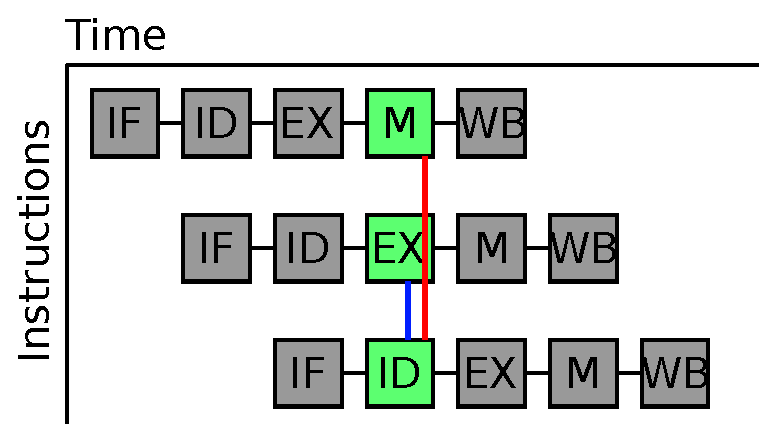
\includegraphics[scale=0.4]{pipeline/data_hazard.eps}
	\label{fig:data_hazard}
	\caption{Time-sheet of the program listed in figure
\ref{fig:data_hazard_code}.}
\end{figure}
The problem is very clear - the data is needed before it is saved at the
appropriate place. However, the data is usually already available in the EX
stage in the ALU, and can therefore be used in the same clock-cycle in the ID
stage. This is called forwarding or bypassing, and is handled by a dedicated
Forwarding Unit. This unit is wired to both EX, MEM and WB stages, and has a
logic unit that checks for matching registers in the instruction, in which case
it forwards the correct result back in the pipeline.

\subsubsection{Control Hazard}
Another type of hazard is the Control Hazard, which occurs when the processor
must make a decision based on an instruction, while others are executing.
Whether a branch is taken or not can be determined by the ALU in the EX stage,
which does a equality check on the two values. This does not add much additional
logic to the circuit, as the forwarding unit already bypasses all the most recent
results as the operands to the ALU. If a branch is taken, a challenge emerges
that we already have the next instructions in both ID and IF stage, even though
our program is inteded to branch away. There are many
possible ways to solve this issue, the most simple, but inefficient one, is to
stall the pipeline by inserting two No-Operation instructions after the branch. This way,
the instruction after the branch will do nothing, but in both situations, we
loose a 2 clock cycles. Although this does not sound like much, considering that
branching instruction make up about 25\% of any assembly code\cite{instruction_frequency},
this can be a lot.\\
A way to ease the problem with this many wasted clock cycles is to move the
branching calculation in the ID stage. A simple comparison unit for the register
values is required, but the forwarding unit also needs to be be modified to
forward results to the ID stage.\\

A better, but much more complex technique to solve this issue, is to have a
dedicated "Prediction" unit in the processor, which will predict whether a branch will be
taken or not, and fetch instructions to the IF stage accordingly.


\subsection{Implementation}
The implementation of the pipelined simulator will group the devices in the
machine together, so that each device or system has its own C structure.

\subsubsection{Simulator structures}
\begin{figure}[H]
	\centering
	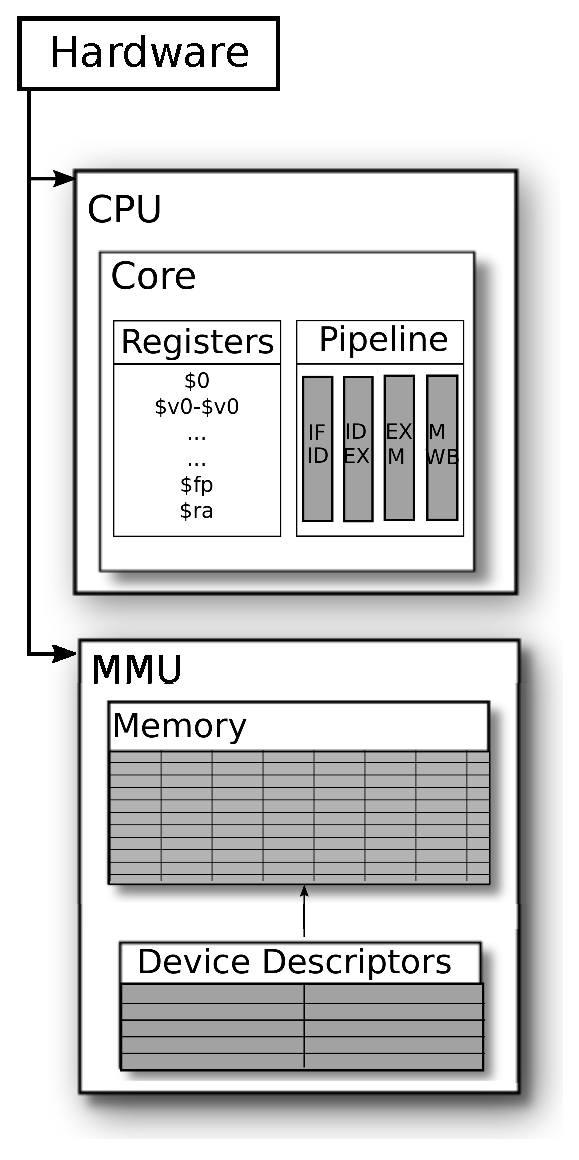
\includegraphics[scale=0.55]{pipeline/structure_layout.eps}
	\caption{Relations between the simulator structures.}
	\label{fig:structure_layout}
\end{figure}
In the simulator, the processor cores, pipeline registers, and memory unit all
belong to a "hardware" structure, that binds them together, making up the state
of the simulated machine. The relations between the components can be seen in figure
\ref{fig:structure_layout}.\\
In the simulator, the hardware structure will be used to pass along the
simulated hardware to functions, which then can access the underlying devices,
modifying them properly.

\subsubsection{Pipeline functions}
The pipeline is implemented by running each pipeline stage separately. For each
clock-tick, the pipeline stage functions are being called in reverse. This can
seem very unnatural, but this prevents pipeline registers to be overwritten
before they are used. This also prevents an instruction to get throught the
pipeline in one tick of the clock, and simplifies the assignment of the pipeline
registers.
\begin{verbatim}
void tick() {
        interpret_wb(...);
        interpret_mem(...);
        interpret_ex(...);
        interpret_id(...);
        interpret_if(...);
}
\end{verbatim}

Each of the functions receive the relevant pointer to the CPU core structure,
which holds all the relevant information about the state of the core.


\subsubsection{Forwarding Unit}
The pipeline stages work without regard for data hazards, which is where data
is required for an instruction before it is stored by the previous instruction.
Therefore, we add a forwarding unit function \texttt{forwarding\_unit()}, which
is run by the end of each clock cycle. Being the last function, it has all the
recent information in all the pipeline stages, which enables it to decide which
values need to be forwarded.\\
The forwarding unit only forwards values to the ALU input mutual exclusion
units MUX A and MUX B. It does that by first checking if the previous
instructions write to a register, that is, modify a register value. If it
indeed is the case, the destination registers are compared, and if the match,
the value from the previous instruction is bypassed. This is done for both the
A and B input to the ALU in both Memory- and Writeback-stages. The code for
forwarding values from stage MEM to EX can be seen in figure
\ref{fig:forwarding_unit_code}. Forwarding from the WB stage is almost
identical.

\begin{figure}[H]
\centering
\begin{lstlisting}[style=customc]
/* Forward to A MUX */
if(EX_MEM.c_reg_write == 1
   && EX_MEM.reg_dst != 0
   && EX_MEM.reg_dst == ID_EX.rs)
       ID_EX.rs_value = EX_MEM.alu_res;

/* Forward to B MUX */
if(EX_MEM.c_reg_write == 1
   && EX_MEM.reg_dst != 0
   && EX_MEM.reg_dst == ID_EX.rt)
      ID_EX.rt_value = EX_MEM.alu_res;
\end{lstlisting}
\caption{ALU result being forwarded from the MEM stage to EX.}
\label{fig:forwarding_unit_code}
\end{figure}

\subsubsection{Hazard detection unit}
Control hazards arise when the processor is branching to another execution path
based on the result of the previous instructions. As there is no "correct"
solution to the branching hazard, the MIPS CPU manufacturers often implement
their own branch predictions based on the intended use of the processor. For
simplicity in our simulator, we will always predict that the branch is
\textit{not} taken. We will also simulate that the branching is decided in the
ID stage\footnote{Technically, we are deciding this in the \texttt{interp\_ex} function,
but this will have the same effect due to the reverse execution of our pipeline stages.}, so that only we only have 1 branch delay slot.
In that case, we always run the next instruction after the
branch. This works well, because this is a widely accepted approach in many
RISC architectures\cite{wiki:branch_delay_slots}.  Knowing that the instruction
following a branch is always executed, many standard compilers and assemblers
restructure the code so that branch-delay slot is not wasted.\\
For example, where assignment of a value to a register and a branch would
consume 3 instructions, utilization of the branch-delay slot can bring it back
to 2. The difference can be seen on figure \ref{fig:branch_delay_slot_compare}.
Note that the order of the instruction does not matter in that case.
\begin{figure}[H]
    \centering
    \begin{subfigure}[t]{0.23\textwidth}
    \begin{lstlisting}[numbers=none]
addi $v0, $0, 10
beq $0, $0, exit
nop
    \end{lstlisting}
    \label{fig:non_utilized_branch_delay}

   \end{subfigure}
   % ~ %add desired spacing between images, e. g. ~, \quad, \qquad, \hfill etc.
      %(or a blank line to force the subfigure onto a new line)
    \begin{subfigure}[t]{0.23\textwidth}
     \begin{lstlisting}[numbers=none]
beq $0, $0, exit
addi $v0, $0, 10
# ...
   \end{lstlisting}
        \label{fig:utilized_branch_delay}
    \end{subfigure}
\caption{Wasted branch delay slot (left) and utilized branch delay slot (right).}
\label{fig:branch_delay_slot_compare}
\end{figure}


